\documentclass{beamer}
\usepackage[utf8]{inputenc}
\usepackage{amsmath}
\usepackage{graphicx}
\usepackage{xcolor}
\usepackage{tikz}

\usetheme{Madrid}
\usecolortheme{default}

% Define custom colors inspired by Star Trek DS9
\definecolor{ds9blue}{RGB}{25,25,112} % Midnight Blue
\definecolor{ds9gold}{RGB}{218,165,32} % Goldenrod
\definecolor{ds9grey}{RGB}{105,105,105} % Dim Gray
\definecolor{ds9red}{RGB}{178,34,34} % Firebrick

% Customize the colors
\setbeamercolor{title}{fg=ds9gold}
\setbeamercolor{frametitle}{bg=ds9blue, fg=white}
\setbeamercolor{block title}{bg=ds9gold, fg=black}
\setbeamercolor{block body}{bg=ds9grey!20, fg=black}
\setbeamercolor{section in toc}{fg=ds9gold}
\setbeamercolor{subsection in toc}{fg=ds9gold!70}
\setbeamercolor{footline}{bg=ds9blue, fg=white}
\setbeamercolor{author in head/foot}{fg=white}
\setbeamercolor{date in head/foot}{fg=white}
\setbeamercolor{title in head/foot}{fg=white}

% Title page configuration
\title[Inclined Planes]{PHYS11 CH:5.4}
\subtitle{Static and Kinetic Friction}
\author[Mr. Gullo]{Mr. Gullo}
\date[Nov 2024]{November 2024}

% Table of contents at the beginning of each section
\AtBeginSection[]
{
  \begin{frame}
    \frametitle{Table of Contents}
    \tableofcontents[currentsection]
  \end{frame}
}

% Add logo
\logo{
\includegraphics[width=0.1\linewidth]{cinec_logo.png}}

\begin{document}

\frame{\titlepage}

\section{Introduction to Friction}

\begin{frame}
\frametitle{Types of Friction}
\begin{itemize}
    \item \textbf{Friction}: Force that opposes motion
    \item Two main types:
    \begin{itemize}
        \item \textbf{Static Friction}: Acts on objects at rest
        \item \textbf{Kinetic Friction}: Acts on objects in motion
    \end{itemize}
    \item Maximum static friction is usually greater than kinetic friction
\begin{figure}[H]
    \centering
    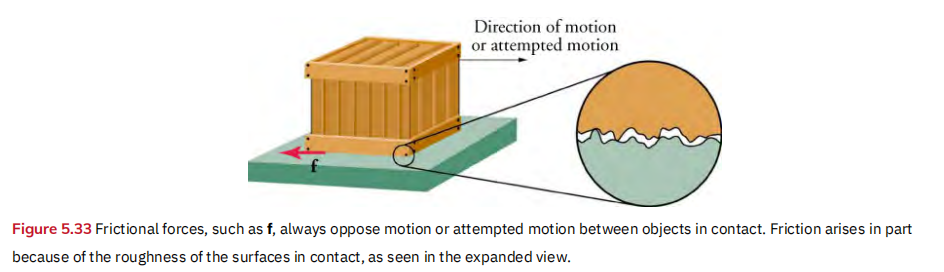
\includegraphics[width=0.8\linewidth]{CH5.4/Screenshot 2024-11-11 110912.png}
\end{figure}
    
\end{itemize}
\end{frame}

\begin{frame}
\frametitle{Friction Formulas}
\begin{block}{Static Friction}
\[ f_s \leq \mu_s N \]
where:
\begin{itemize}
    \item $f_s$ is static friction force
    \item $\mu_s$ is coefficient of static friction
    \item $N$ is normal force
\end{itemize}
\end{block}

\begin{block}{Kinetic Friction}
\[ f_k = \mu_k N \]
where:
\begin{itemize}
    \item $f_k$ is kinetic friction force
    \item $\mu_k$ is coefficient of kinetic friction
\end{itemize}
\end{block}
\end{frame}

\begin{frame}
\frametitle{Coefficients of Friction}
\begin{table}
\begin{tabular}{|l|c|c|}
\hline
System & Static Friction & Kinetic Friction \\
\hline
Rubber on dry concrete & 1.0 & 0.7 \\
Wood on wood & 0.5 & 0.3 \\
Steel on steel (dry) & 0.6 & 0.3 \\
Steel on steel (oiled) & 0.05 & 0.03 \\
Ice on ice & 0.1 & 0.03 \\
\hline
\end{tabular}
\end{table}
\end{frame}

\section{Inclined Planes}

\begin{frame}
\frametitle{Forces on an Inclined Plane}
\begin{itemize}
    \item Weight components on an incline:
    \begin{itemize}
        \item Parallel to slope: $w_\parallel = mg\sin\theta$
        \item Perpendicular to slope: $w_\perp = mg\cos\theta$
    \end{itemize}
    \item Normal force ($N$) equals perpendicular component
    \item Friction acts parallel to surface, opposing motion
\begin{figure}[H]
    \centering
    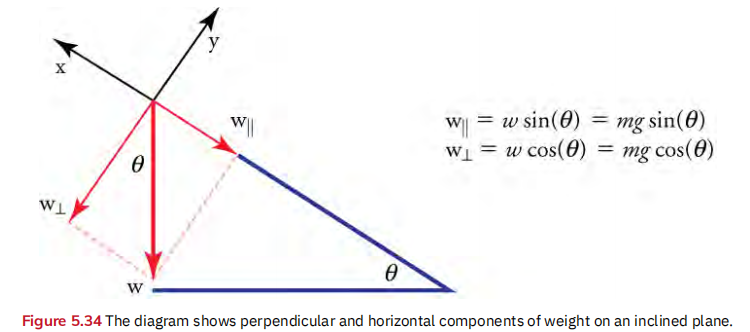
\includegraphics[width=0.7\linewidth]{CH5.4/Screenshot 2024-11-11 110923.png}
\end{figure}
\end{itemize}
\end{frame}

\begin{frame}
\frametitle{Problem Solving Steps}
1. Draw a sketch of the problem
\vspace{0.5em}

2. Identify known and unknown quantities
\vspace{0.5em}

3. Draw free-body diagram with rotated coordinate system
\vspace{0.5em}

4. Apply Newton's second law:
\begin{itemize}
    \item If no acceleration: $F_{net} = 0$
    \item If accelerating: $F_{net} = ma$
\end{itemize}
\vspace{0.5em}

5. Check answer for reasonableness
\end{frame}

\section{Example Problems}

\begin{frame}
\frametitle{Example: Skier on a Slope}
\begin{block}{Problem}
A 62 kg skier slides down a snowy slope at 25°. Find $\mu_k$ if friction is 45.0 N.
\end{block}
\begin{figure}[H]
    \centering
    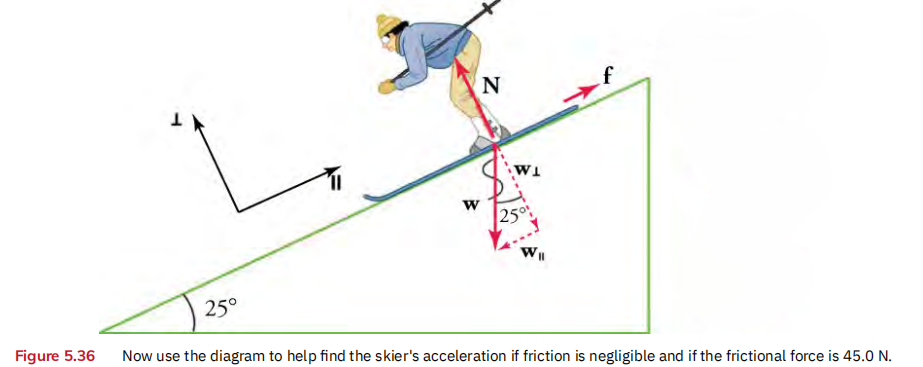
\includegraphics[width=0.8\linewidth]{CH5.4/Screenshot 2024-11-11 110959SansFBD.png}
\end{figure}
\end{frame}

\begin{frame}
\begin{figure}[H]
    \centering
    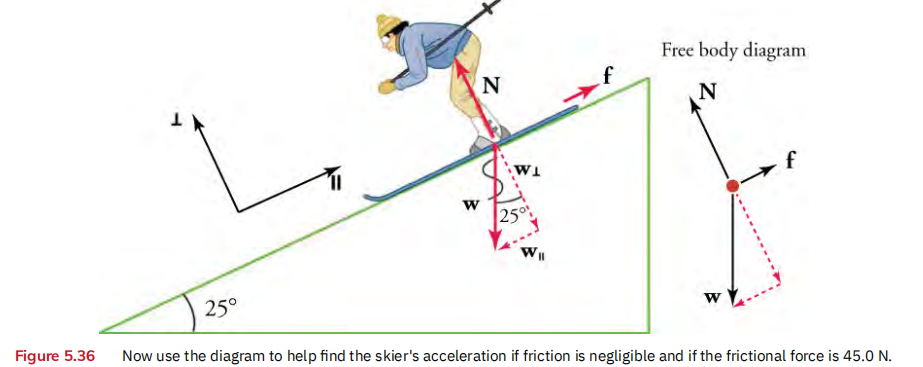
\includegraphics[width=1\linewidth]{CH5.4/Screenshot 2024-11-11 110959.png}
\end{figure}

\end{frame}

\begin{frame}
\begin{figure}[H]
    \centering
    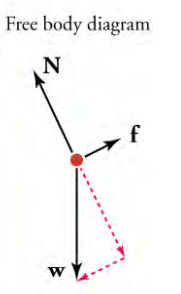
\includegraphics[width=.2\linewidth]{CH5.4/Screenshot 2024-11-11 111003.png}
\end{figure}

\begin{block}{Solution}
\[ N = mg\cos\theta = (62\text{ kg})(9.80\text{ m/s}^2)\cos(25°) \]
\[ f_k = \mu_k N = 45.0\text{ N} \]
\[ \mu_k = \frac{f_k}{N} = \frac{45.0\text{ N}}{551\text{ N}} = 0.082 \]
\end{block}
\end{frame}

\begin{frame}
\frametitle{Example: Acceleration on an Incline}
\begin{block}{Problem - Part A}
What is the skier's acceleration if friction is negligible?
\end{block}
\begin{block}{Solution}
\[ a = g\sin\theta \]
\[ a = (9.80\text{ m/s}^2)\sin(25°) = 4.14\text{ m/s}^2 \]
\end{block}
\end{frame}

\begin{frame}
\frametitle{Example: Acceleration with Friction}
\begin{block}{Problem - Part B}
What is the skier's acceleration with 45.0 N friction?
\end{block}
\begin{block}{Solution}
\[ F_{net} = mg\sin\theta - f_k \]
\[ a = g\sin\theta - \frac{f_k}{m} \]
\[ a = 9.80\sin(25°) - \frac{45.0}{60.0} = 3.39\text{ m/s}^2 \]
\end{block}
\end{frame}

\section{Check Your Understanding}

\begin{frame}
\frametitle{Review Questions}
\begin{enumerate}
    \item What is friction?
    \begin{itemize}
        \item An external force that opposes relative motion
    \end{itemize}
    
    \item Compare static vs. kinetic friction:
    \begin{itemize}
        \item Static: Acts on objects at rest
        \item Kinetic: Acts on objects in motion
        \item Static friction maximum $>$ Kinetic friction
    \end{itemize}
\end{enumerate}
\end{frame}


\begin{frame}

\end{frame}


\begin{frame}
    \begin{itemize}
        \item Static friction maximum $>$ Kinetic friction
    \end{itemize}
\begin{figure}[H]
    \centering
    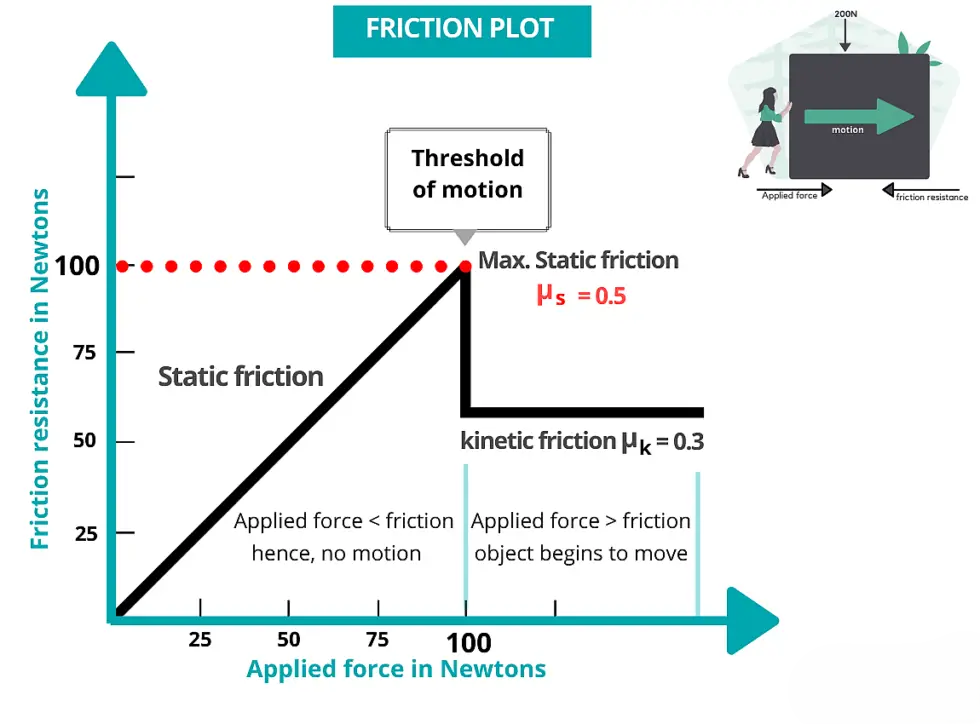
\includegraphics[width=0.9\linewidth]{CH5.4/Friction-Plot-980x724.png}
\end{figure}
\end{frame}

\end{document}